%!TEX program = xelatex
\documentclass[11pt]{beamer}

\usepackage{amsfonts}
\usepackage{amsmath}
\usepackage{blindtext}
\usepackage{enumitem}
\usepackage{fancyvrb}
\usepackage{tikz}

\usetheme{SaoPaulo}

\title{Numerical Python}
\subtitle{optimization}
\author{CS101 Lecture \#18}
\date{2016-11-23}

\setcounter{showSlideNumbers}{1}

\newcommand{\correctstar}{\textcolor{red}{$\star$}}

\begin{document}
  \setcounter{showProgressBar}{0}
  \setcounter{showSlideNumbers}{0}

%%%%%%%%%%%%%%%%%%%%%%%%%%%%%%%%%%%%%%%%%%%%%%%%%%%%%%%%%%%%%%%%%%%%%%%%%%%%%%%%
\frame{\titlepage}

%%%%%%%%%%%%%%%%%%%%%%%%%%%%%%%%%%%%%%%%%%%%%%%%%%%%%%%%%%%%%%%%%%%%%%%%%%%%%%%%
\setcounter{framenumber}{0}
\setcounter{showProgressBar}{1}
\setcounter{showSlideNumbers}{1}


\iffalse
%%%%%%%%%%%%%%%%%%%%%%%%%%%%%%%%%%%%%%%%%%%%%%%%%%%%%%%%%%%%%%%%%%%%%%%%%%%%%%%%
\section{Administrivia}

%%%%%%%%%%%%%%%%%%%%%%%%%%%%%%%%%%%%%%%%%%%%%%%%%%%%%%%%%%%%%%%%%%%%%%%%%%%%%%%%
\begin{frame}
  \frametitle{Administrivia}
  \Enlarge

  \begin{itemize}
  \myitem  Homework \#9 is due Friday, Dec.\ 9.
  \myitem  Homework \#10 is due Tuesday, Dec.\ 20.
  \myitem  Midterm \#2 is Monday, Dec. 19 from 7–10 p.m.
  \end{itemize}
\end{frame}

\fi


\iffalse
%%%%%%%%%%%%%%%%%%%%%%%%%%%%%%%%%%%%%%%%%%%%%%%%%%%%%%%%%%%%%%%%%%%%%%%%%%%%%%%%
\section{Warmup Question}

%%%%%%%%%%%%%%%%%%%%%%%%%%%%%%%%%%%%%%%%%%%%%%%%%%%%%%%%%%%%%%%%%%%%%%%%%%%%%%%%
\begin{frame}[fragile]
  \frametitle{Question \#1}

  \begin{Verbatim}
def fact( n ):
    if n <= 1:
        return 1
    else:
        ???
  \end{Verbatim}

Which line of code correctly makes \texttt{fact} return the factorial $n!$?

  \begin{enumerate}[label=\Alph*]
    \item  \texttt{return fact( n - 1 ) * fact( n )}
    \item  \texttt{return fact( n - 1 ) * n}
    \item  \texttt{return ( n - 1 ) * n}
    \item  \texttt{return fact( n - 2 ) * n}
  \end{enumerate}
\end{frame}

%%%%%%%%%%%%%%%%%%%%%%%%%%%%%%%%%%%%%%%%%%%%%%%%%%%%%%%%%%%%%%%%%%%%%%%%%%%%%%%%
\begin{frame}[fragile]
  \frametitle{Question \#1}

  \begin{Verbatim}
def fact( n ):
    if n <= 1:
        return 1
    else:
        ???
  \end{Verbatim}

Which line of code correctly makes \texttt{fact} return the factorial $n!$?

  \begin{enumerate}[label=\Alph*]
    \item  \texttt{return fact( n - 1 ) * fact( n )}
    \item  \texttt{return fact( n - 1 ) * n}  \correctstar
    \item  \texttt{return ( n - 1 ) * n}
    \item  \texttt{return fact( n - 2 ) * n}
  \end{enumerate}
\end{frame}

\fi
%%%%%%%%%%%%%%%%%%%%%%%%%%%%%%%%%%%%%%%%%%%%%%%%%%%%%%%%%%%%%%%%%%%%%%%%%%%%%%%%
\section{Randomness Refresher}

%%%%%%%%%%%%%%%%%%%%%%%%%%%%%%%%%%%%%%%%%%%%%%%%%%%%%%%%%%%%%%%%%%%%%%%%%%%%%%%%
\begin{frame}[fragile]
  \frametitle{Randomness refresher}
  \Enlarge

  \begin{enumerate}
  \myitem  \texttt{randint( start,end,size=tuple )} %\pause
  \myitem  \texttt{uniform( start,end,size=tuple )} %\pause
  \myitem  \texttt{randn(d1,d2,..)}    \#specify size of output %\pause
  \mysubitem  Note that the interfaces for each are slightly different.
  \end{enumerate}
\end{frame}

%%%%%%%%%%%%%%%%%%%%%%%%%%%%%%%%%%%%%%%%%%%%%%%%%%%%%%%%%%%%%%%%%%%%%%%%%%%%%%%%
\begin{frame}[fragile]
  \frametitle{Question \#1}
  \Enlarge

  \begin{Verbatim}
x = np.random.randint( 0,10, size=(1000,1) )
plt.hist( x )
plt.show()
  \end{Verbatim}

  What is a possible output of this code?

  \begin{center}
  \begin{tabular}{ccc}
    A & B & C \\
    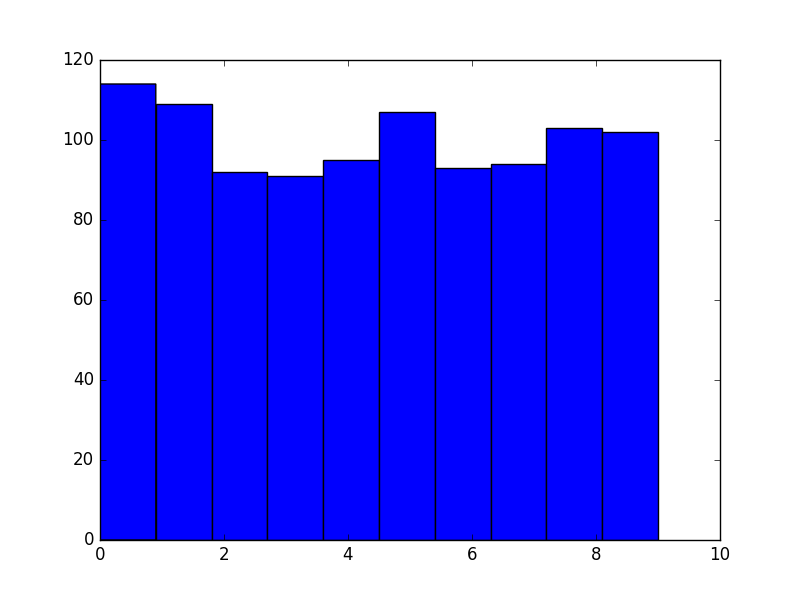
\includegraphics[width=0.25\textwidth]{./img/figure_1.png}
    &
    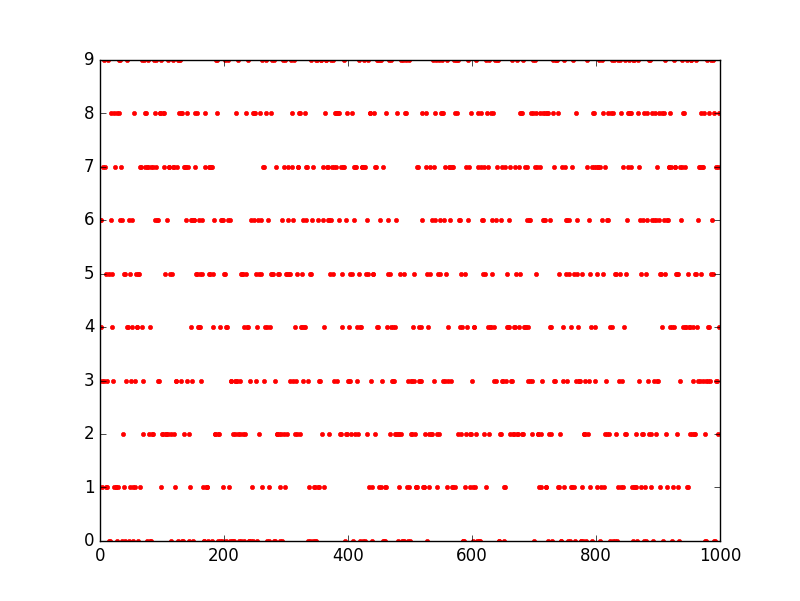
\includegraphics[width=0.25\textwidth]{./img/figure_2.png}
    &
    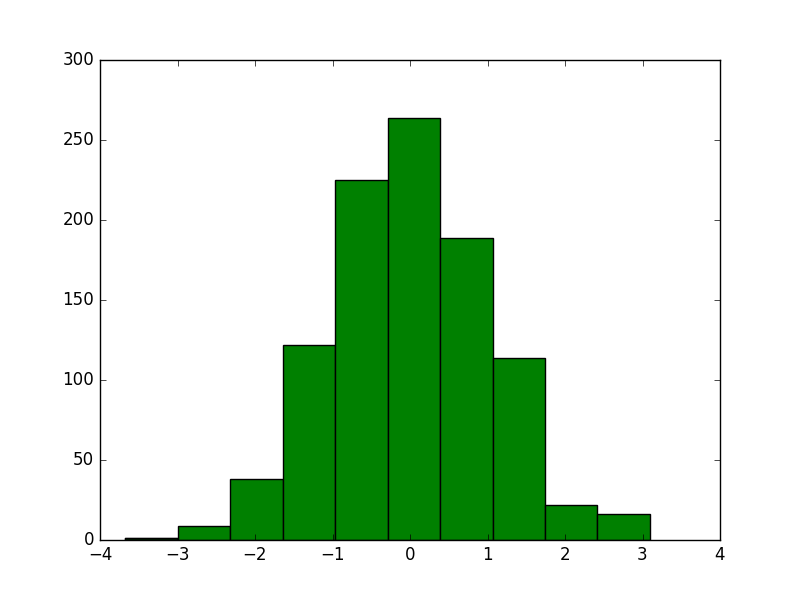
\includegraphics[width=0.25\textwidth]{./img/figure_3.png}
  \end{tabular}
  \end{center}
\end{frame}

%%%%%%%%%%%%%%%%%%%%%%%%%%%%%%%%%%%%%%%%%%%%%%%%%%%%%%%%%%%%%%%%%%%%%%%%%%%%%%%%
\begin{frame}[fragile]
  \frametitle{Question \#1}
  \Enlarge

  \begin{Verbatim}
x = np.random.randint( 0,10, size=(1000,1) )
plt.hist( x )
plt.show()
  \end{Verbatim}

  What is a possible output of this code?

  \begin{center}
  \begin{tabular}{ccc}
    A & B & C \\
    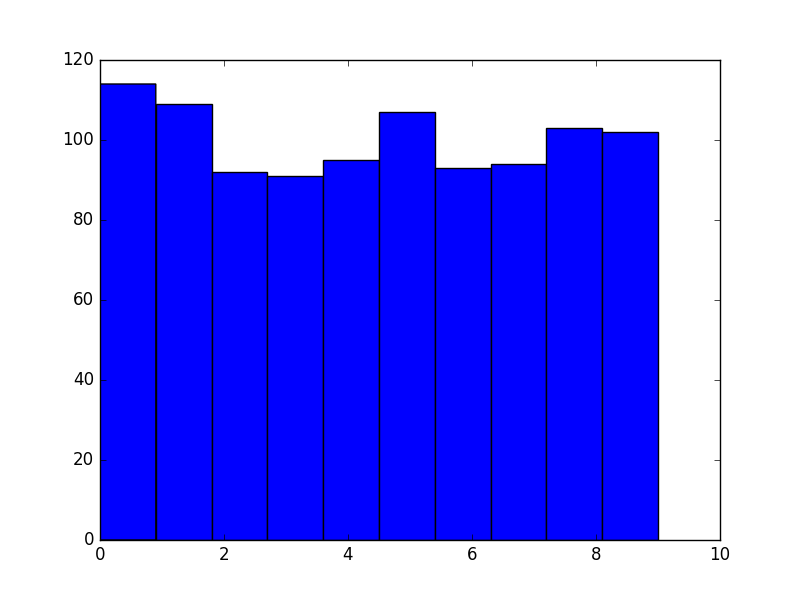
\includegraphics[width=0.25\textwidth]{./img/figure_1.png}
    &
    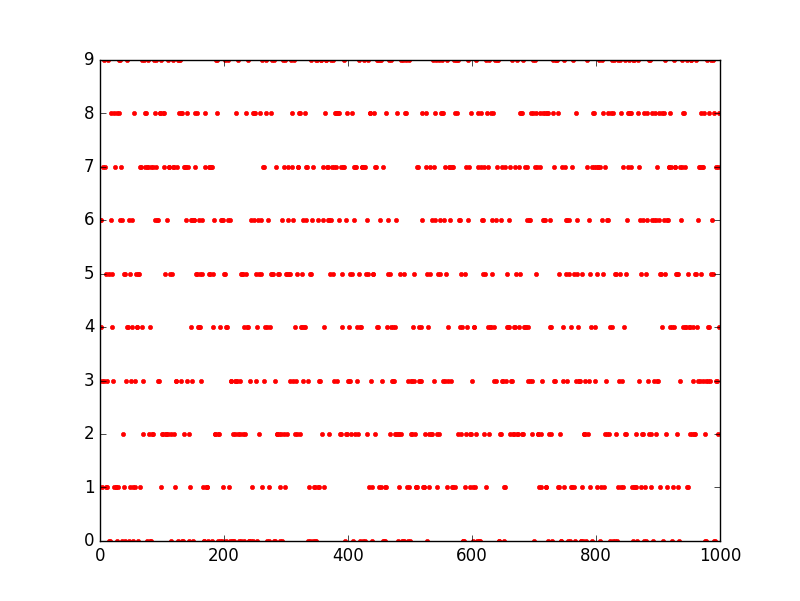
\includegraphics[width=0.25\textwidth]{./img/figure_2.png}
    &
    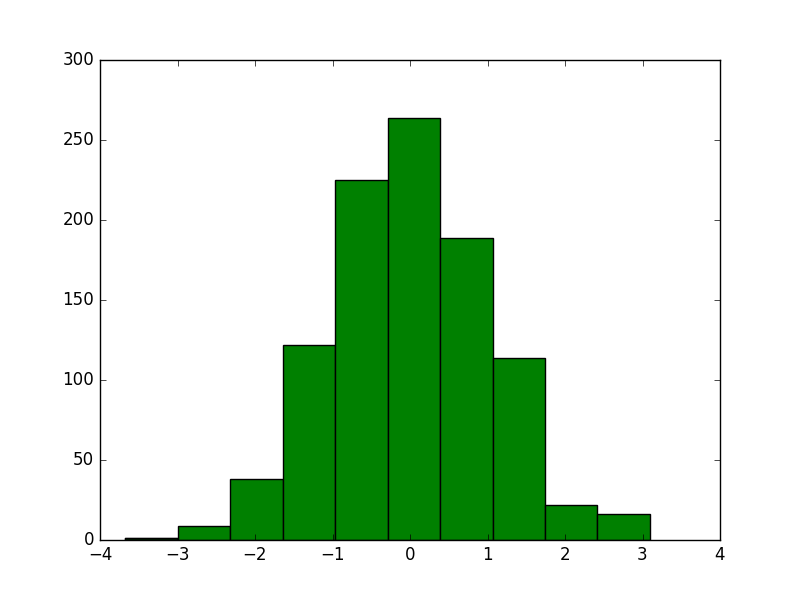
\includegraphics[width=0.25\textwidth]{./img/figure_3.png}
    \\
    \correctstar & & \\
  \end{tabular}
  \end{center}
\end{frame}

%%%%%%%%%%%%%%%%%%%%%%%%%%%%%%%%%%%%%%%%%%%%%%%%%%%%%%%%%%%%%%%%%%%%%%%%%%%%%%%%
\begin{frame}[fragile]
  \frametitle{Question \#2}
  \Enlarge

  \begin{Verbatim}
x = np.random.uniform( size=(1000,1) )
plt.plot( x, 'c.' )
plt.ylim( (-1,2) )
plt.show()
  \end{Verbatim}

  What is a possible output of this code?

  \begin{center}
  \begin{tabular}{cccc}
    A & B & C & D \\
    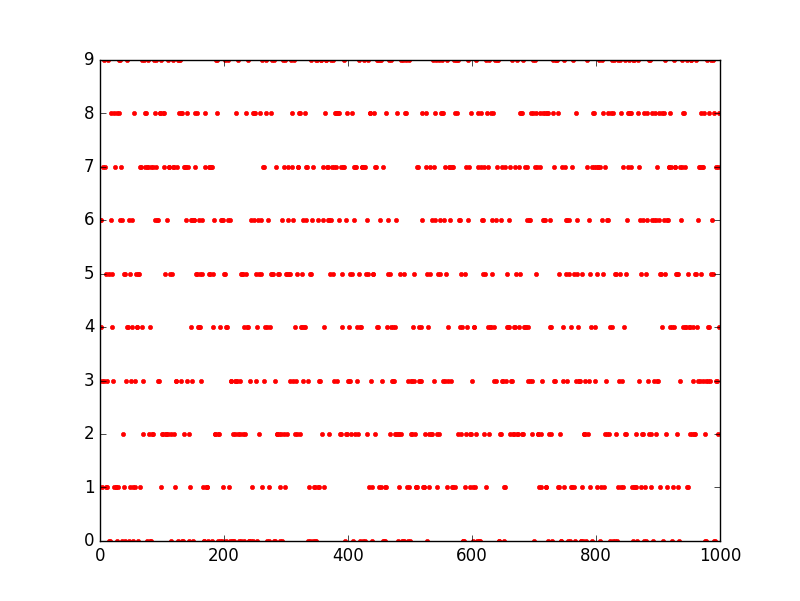
\includegraphics[width=0.25\textwidth]{./img/figure_2.png}
    &
    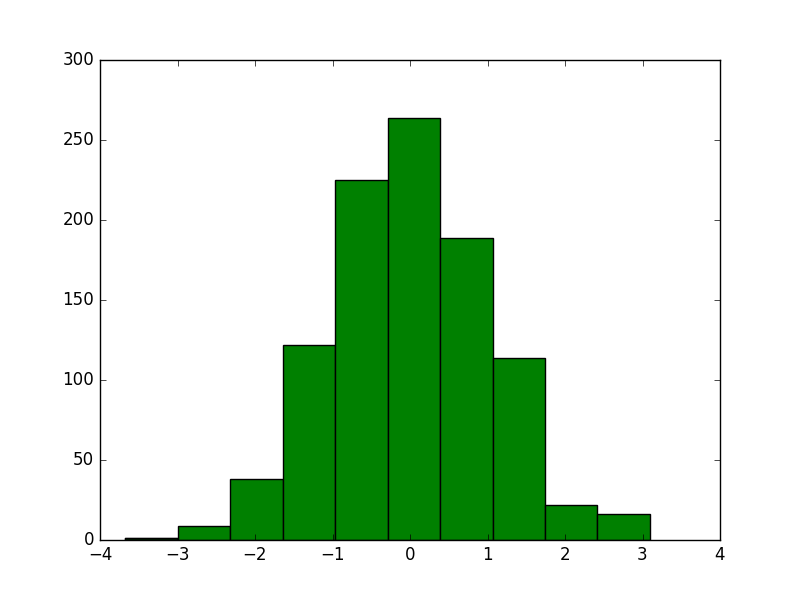
\includegraphics[width=0.25\textwidth]{./img/figure_3.png}
    &
    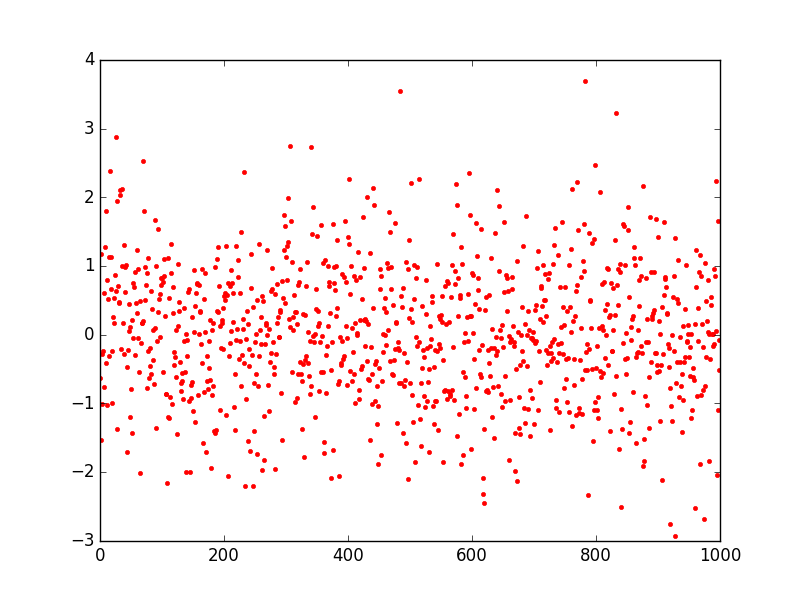
\includegraphics[width=0.25\textwidth]{./img/figure_4.png}
    &
    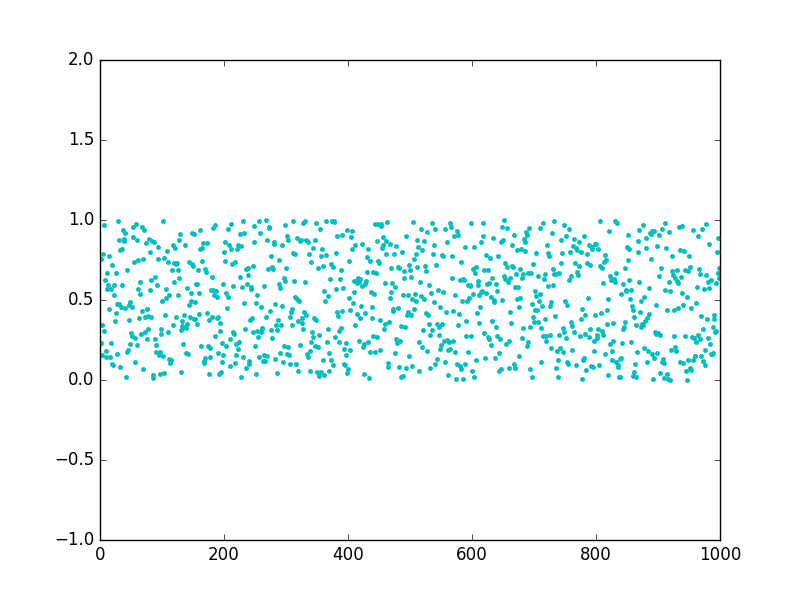
\includegraphics[width=0.25\textwidth]{./img/figure_5.png}
  \end{tabular}
  \end{center}
\end{frame}

%%%%%%%%%%%%%%%%%%%%%%%%%%%%%%%%%%%%%%%%%%%%%%%%%%%%%%%%%%%%%%%%%%%%%%%%%%%%%%%%
\begin{frame}[fragile]
  \frametitle{Question \#2}
  \Enlarge

  \begin{Verbatim}
x = np.random.uniform( size=(1000,1) )
plt.plot( x, 'c.' )
plt.ylim( (-1,2) )
plt.show()
  \end{Verbatim}

  What is a possible output of this code?

  \begin{center}
  \begin{tabular}{cccc}
    A & B & C & D \\
    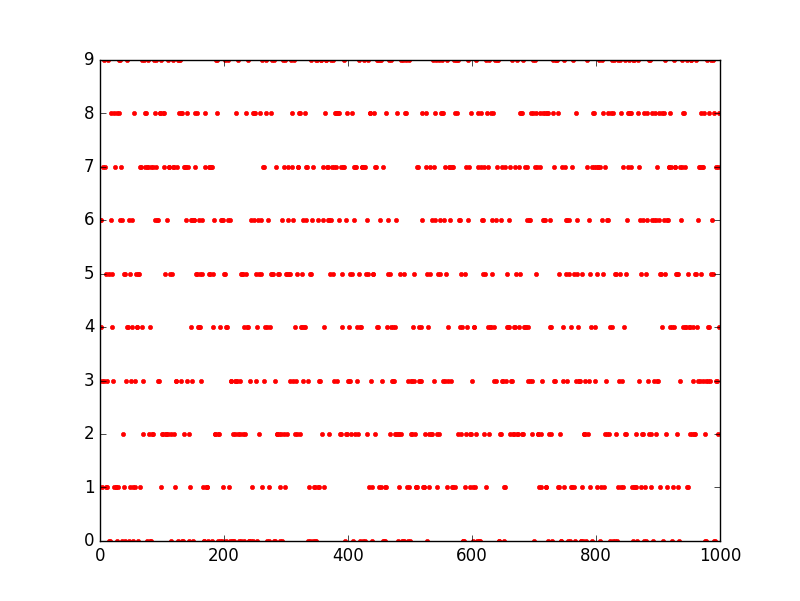
\includegraphics[width=0.25\textwidth]{./img/figure_2.png}
    &
    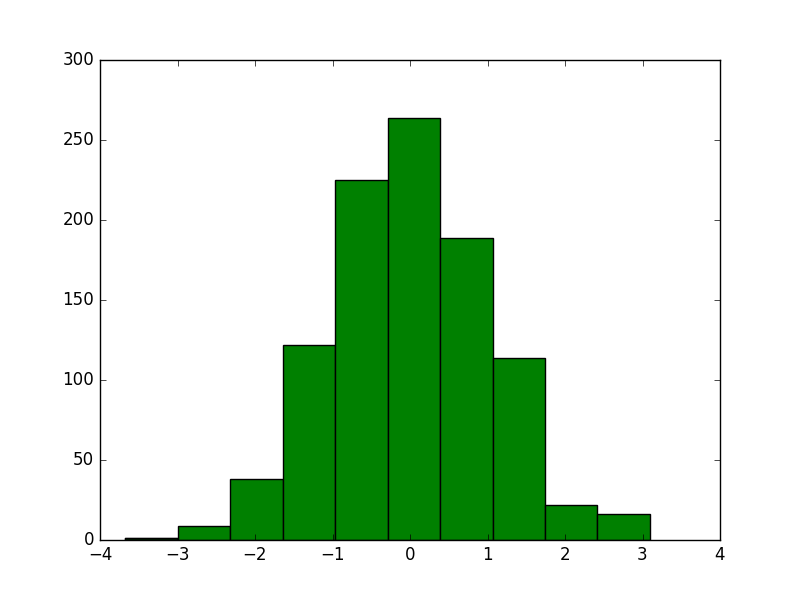
\includegraphics[width=0.25\textwidth]{./img/figure_3.png}
    &
    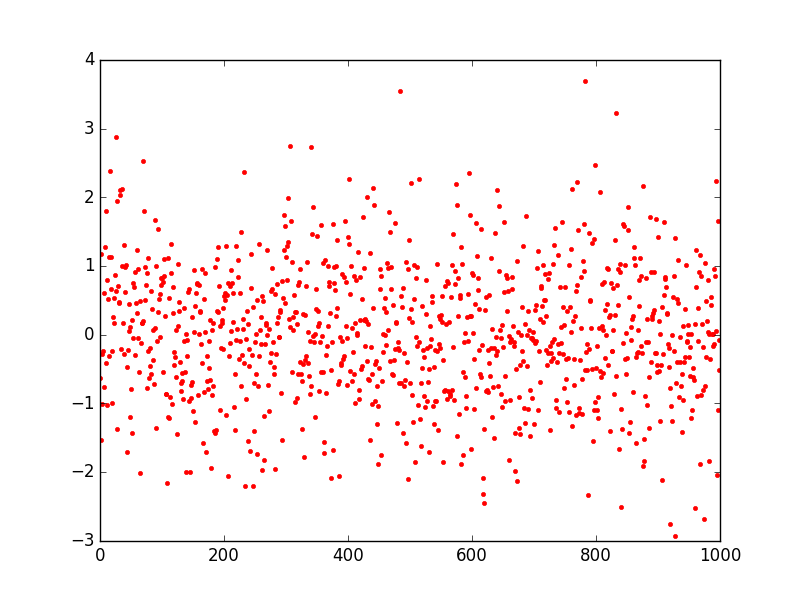
\includegraphics[width=0.25\textwidth]{./img/figure_4.png}
    &
    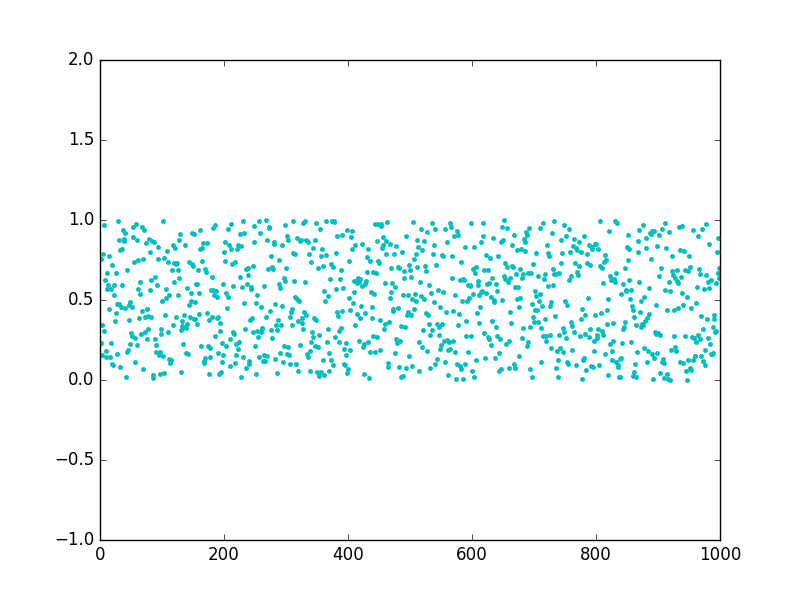
\includegraphics[width=0.25\textwidth]{./img/figure_5.png}
    \\
    & & & \correctstar \\
    
  \end{tabular}
    http://matplotlib.org/api/colors\_api.html
  \end{center}
\end{frame}

%%%%%%%%%%%%%%%%%%%%%%%%%%%%%%%%%%%%%%%%%%%%%%%%%%%%%%%%%%%%%%%%%%%%%%%%%%%%%%%%
\section{Optimization}

%%%%%%%%%%%%%%%%%%%%%%%%%%%%%%%%%%%%%%%%%%%%%%%%%%%%%%%%%%%%%%%%%%%%%%%%%%%%%%%%
\begin{frame}[fragile]
  \frametitle{Optimization}
  \Enlarge

  On vacation, you purchase a range of $n$ souvenirs of varying weight and value.  When it comes time to pack, you find that your bag has a weight limit of 50 pounds.  What is the best set of items to take on the flight?
\end{frame}

%%%%%%%%%%%%%%%%%%%%%%%%%%%%%%%%%%%%%%%%%%%%%%%%%%%%%%%%%%%%%%%%%%%%%%%%%%%%%%%%
\begin{frame}[fragile]
  \frametitle{Optimization}
  \Enlarge

  \begin{enumerate}
  \myitem  Given a function $f(x)$, find $x$ such that $f(x)$ is maximized (or minimized).
  \myitem  The goal is to search the domain for the optimal $x$ yielding the optimal $f(x)$.
  \myitem  Many clever techniques exist, but we'll start with a na\"{i}ve approach.
  \end{enumerate}
\end{frame}

%%%%%%%%%%%%%%%%%%%%%%%%%%%%%%%%%%%%%%%%%%%%%%%%%%%%%%%%%%%%%%%%%%%%%%%%%%%%%%%%
\begin{frame}[fragile]
  \frametitle{Setup}
  \Enlarge

  \begin{Verbatim}
import numpy as np

n = 10
items   = list(range(n))
weights = np.random.uniform( size=(n,1) )*50
values  = np.random.uniform( size=(n,1) )*100
  \end{Verbatim}
\end{frame}

%%%%%%%%%%%%%%%%%%%%%%%%%%%%%%%%%%%%%%%%%%%%%%%%%%%%%%%%%%%%%%%%%%%%%%%%%%%%%%%%
\begin{frame}[fragile]
  \frametitle{Setup}

  \begin{Verbatim}
def f( wts, vals ):
    total_weight = 0
    total_value = 0

    for i in range( len( wts ) ):
        total_weight += wts[ i ]
        total_value  += vals[ i ]

    if total_weight >= 50:
        return 0
    else:
        return total_value
  \end{Verbatim}
\end{frame}

%%%%%%%%%%%%%%%%%%%%%%%%%%%%%%%%%%%%%%%%%%%%S%%%%%%%%%%%%%%%%%%%%%%%%%%%%%%%%%%%
% full-slide image
{ \setbeamertemplate{navigation symbols}{}
\begin{frame}[plain]
%  \Enlarge

  \begin{tikzpicture}[remember picture,overlay]
    \node[at=(current page.center)] {
        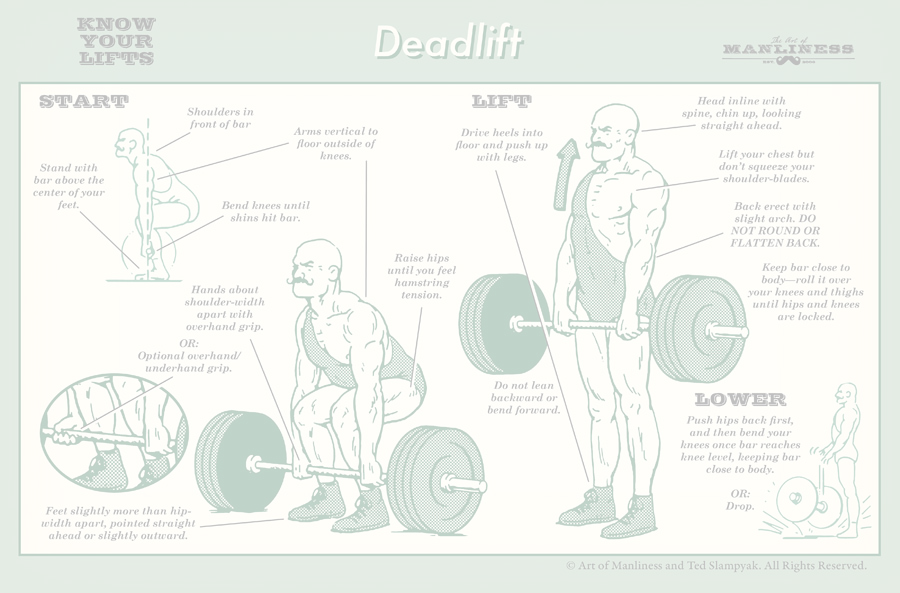
\includegraphics[height=\paperheight]{./img/deadlift.png}
    };
  \end{tikzpicture}

  \begin{enumerate}
  \myitem  Given a function $f(x)$, find $x$ such that $f(x)$ is maximized (or minimized). %\pause
  \myitem  Brute-force searches the \emph{entire} domain of $f$. %\pause
  \myitem  How could we do this in our case?
  \end{enumerate}
 \end{frame}
}

%%%%%%%%%%%%%%%%%%%%%%%%%%%%%%%%%%%%%%%%%%%%%%%%%%%%%%%%%%%%%%%%%%%%%%%%%%%%%%%%
\begin{frame}[fragile]
  \frametitle{Optimization}
  \Enlarge

  \begin{enumerate}
  \myitem  Two useful functions from \texttt{itertools} to keep in mind:
    \begin{enumerate}
    \mysubitem  \texttt{combinations}:  provide all subsets of size \texttt{n}. %\pause
    \mysubitem  \texttt{product}:  replace nested \texttt{for} loops.
    \end{enumerate}
  \end{enumerate}
\end{frame}

%%%%%%%%%%%%%%%%%%%%%%%%%%%%%%%%%%%%%%%%%%%%%%%%%%%%%%%%%%%%%%%%%%%%%%%%%%%%%%%%
\begin{frame}[fragile]
  \frametitle{Optimization}
  \Enlarge

  \begin{enumerate}
  \myitem  \texttt{combinations}:  provide all subsets of size \texttt{n}.
  \end{enumerate}
  \begin{Verbatim}
import itertools

a = [ 1,2,3,4 ]
for x in itertools.combinations( a,2 ):
    print( x )
  \end{Verbatim}
\end{frame}

%%%%%%%%%%%%%%%%%%%%%%%%%%%%%%%%%%%%%%%%%%%%%%%%%%%%%%%%%%%%%%%%%%%%%%%%%%%%%%%%
\begin{frame}[fragile]
  \frametitle{Optimization}
  \Enlarge

  \begin{enumerate}
  \myitem  \texttt{product}:  replace nested \texttt{for} loops.
  \myitem  Can use \texttt{repeat=n} argument as well.
  \end{enumerate}
  \begin{Verbatim}
import itertools

a = [ 1,2,3,4 ]
b = [ 'g','h','i' ]
for x in itertools.product( a,b ):
    print( x )
for x in itertools.product( a, repeat=3 ):
    print( x )
  \end{Verbatim}
\end{frame}

%%%%%%%%%%%%%%%%%%%%%%%%%%%%%%%%%%%%%%%%%%%%%%%%%%%%%%%%%%%%%%%%%%%%%%%%%%%%%%%%
\begin{frame}[fragile]
  \frametitle{Question \#3}

  \begin{Verbatim}
x = 'ABCD'
z = 'XYZ'

for a in itertools.product( x,y ):
    print( ' '.join( a ) )
  \end{Verbatim}

Which of the following is \emph{not} printed?

  \begin{enumerate}[label=\Alph*]
    \item  \texttt{'A X'}
    \item  \texttt{'B D'}
    \item  \texttt{'C X'}
    \item  \texttt{'D Z'}
  \end{enumerate}
\end{frame}

%%%%%%%%%%%%%%%%%%%%%%%%%%%%%%%%%%%%%%%%%%%%%%%%%%%%%%%%%%%%%%%%%%%%%%%%%%%%%%%%
\begin{frame}[fragile]
  \frametitle{Question \#4}

  \begin{Verbatim}
x = 'ABCD'
z = 'XYZ'

for a in itertools.product( x,y ):
    print( ' '.join( a ) )
  \end{Verbatim}

Which of the following is \emph{not} printed?

  \begin{enumerate}[label=\Alph*]
    \item  \texttt{'A X'}
    \item  \texttt{'B D'}  \correctstar
    \item  \texttt{'C X'}
    \item  \texttt{'D Z'}
  \end{enumerate}
\end{frame}

%%%%%%%%%%%%%%%%%%%%%%%%%%%%%%%%%%%%%%%%%%%%%%%%%%%%%%%%%%%%%%%%%%%%%%%%%%%%%%%%
\begin{frame}[fragile]
  \frametitle{Setup}

  \begin{Verbatim}
import itertools

max_value = 0.0
max_set = None
for i in range(1,n+1):
    for set in itertools.combinations( items,i ):
        wts  = []
        vals = []
        for item in set:
            wts.append( weights[ item ] )
            vals.append( values[ item ] )
        value = f( wts,vals )
        if value > max_value:
            max_value = value
            max_set = set
  \end{Verbatim}
\end{frame}

%%%%%%%%%%%%%%%%%%%%%%%%%%%%%%%%%%%%%%%%%%%%%%%%%%%%%%%%%%%%%%%%%%%%%%%%%%%%%%%%
\begin{frame}[fragile]
  \frametitle{Optimization}

  \begin{enumerate}
  \myitem  Brute-force search of a password: %\pause
  \end{enumerate}
  \begin{Verbatim}
def check_password( pwd ):
    if pwd == 'pas':
        return True
    else:
        return False

chars = 'ABCDEFGHIJKLMNOPQRSTUVWXYZ'+\
        'abcdefghijklmnopqrstuvwxyz0123456789'
for pair in itertools.product( chars, repeat=3 ):
    pair = ''.join( pair )
    if check_password( pair ):
        print( pair )
  \end{Verbatim}
\end{frame}

%%%%%%%%%%%%%%%%%%%%%%%%%%%%%%%%%%%%%%%%%%%%%%%%%%%%%%%%%%%%%%%%%%%%%%%%%%%%%%%
\begin{frame}[fragile]
  \frametitle{Optimization}
  \Enlarge

  \begin{enumerate}
  \myitem  Brute-force search of a password: %\pause
  \end{enumerate}
  $$
  \begin{array}{ll}
      & 2 \times n(\textrm{alphabet}) + n(\textrm{digits}) + n(\textrm{special}) \\
    = & 2 \times 26 + 10 + \{24\textrm{--}32\} \\
    = & \{86\textrm{--}94\}
  \end{array}
  $$
  %\pause
  \emph{per letter!}  This gets very big very quickly!
\end{frame}

\iffalse
%%%%%%%%%%%%%%%%%%%%%%%%%%%%%%%%%%%%%%%%%%%%%%%%%%%%%%%%%%%%%%%%%%%%%%%%%%%%%%%%
\begin{frame}
	\frametitle{Administrivia}
	\Enlarge
	
	\begin{itemize}
		\myitem  Homework \#9 is due Friday, Dec.\ 9.
		\myitem  Homework \#10 is due Tuesday, Dec.\ 20.
		\myitem  Midterm \#2 is Monday, Dec. 19 from 7–10 p.m.
	\end{itemize}
\end{frame}

\fi

\end{document}
